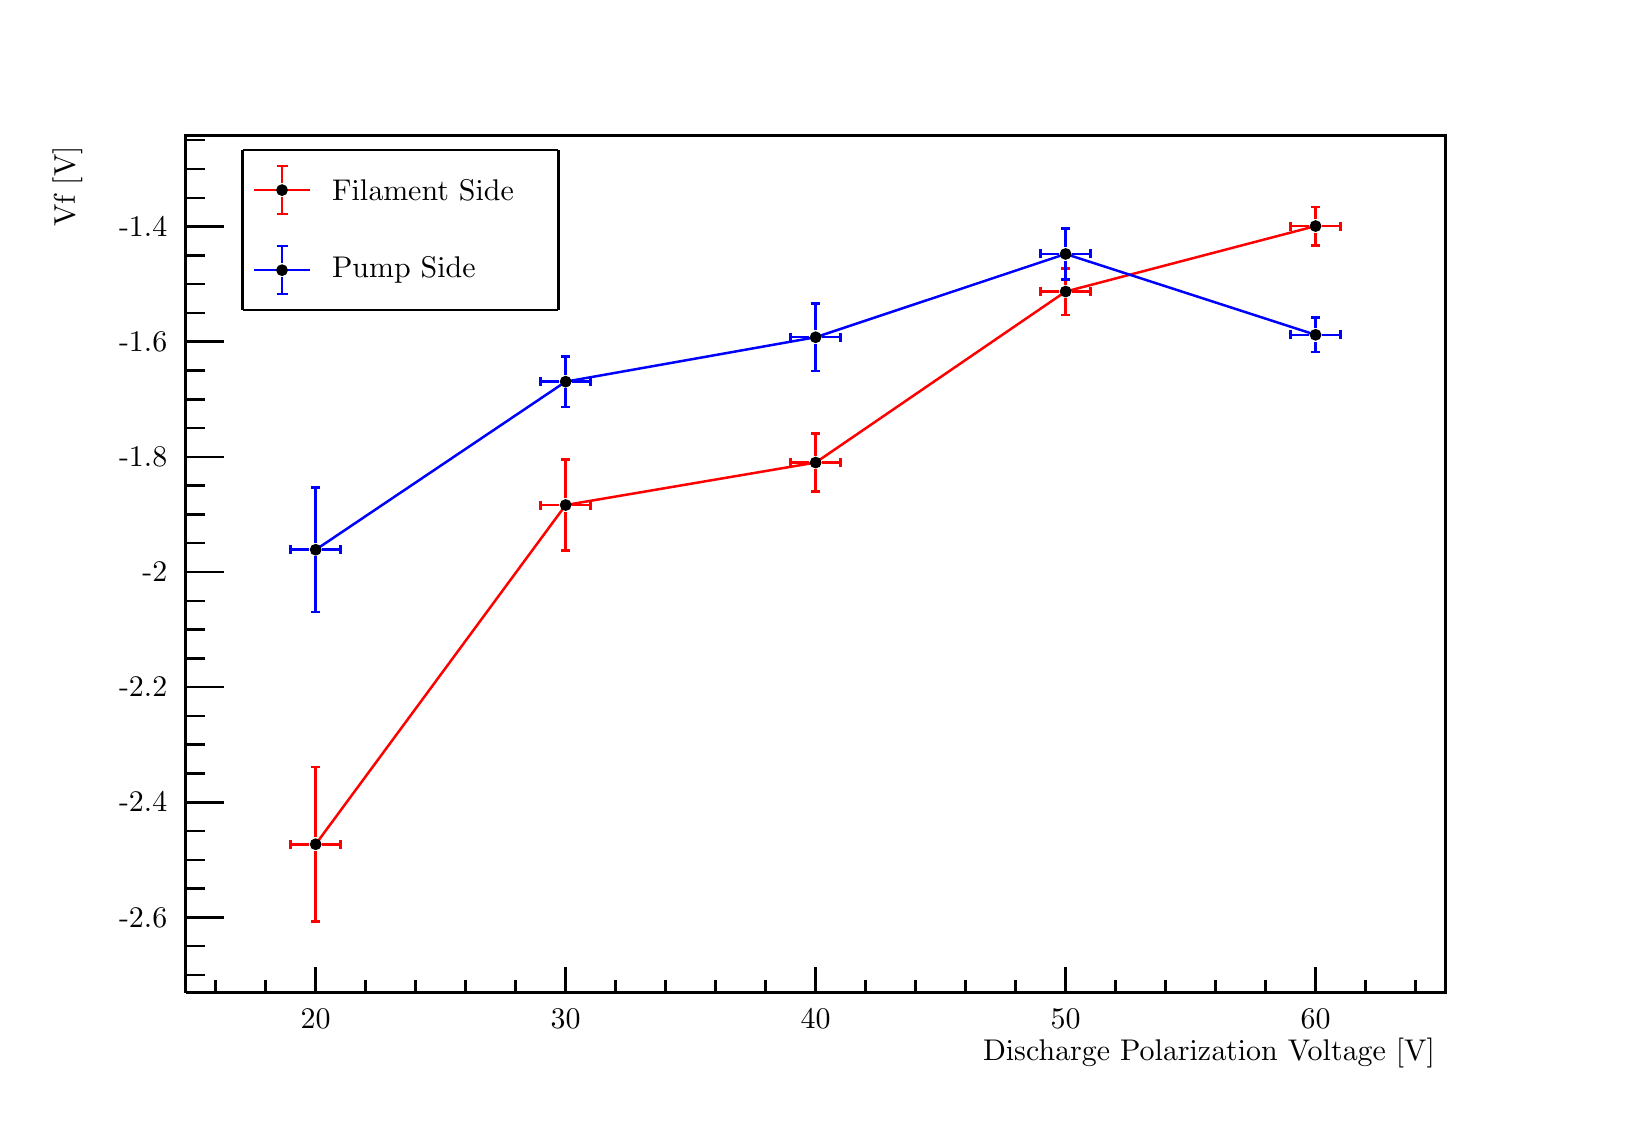
\begin{tikzpicture}
\pgfdeclareplotmark{cross} {
\pgfpathmoveto{\pgfpoint{-0.3\pgfplotmarksize}{\pgfplotmarksize}}
\pgfpathlineto{\pgfpoint{+0.3\pgfplotmarksize}{\pgfplotmarksize}}
\pgfpathlineto{\pgfpoint{+0.3\pgfplotmarksize}{0.3\pgfplotmarksize}}
\pgfpathlineto{\pgfpoint{+1\pgfplotmarksize}{0.3\pgfplotmarksize}}
\pgfpathlineto{\pgfpoint{+1\pgfplotmarksize}{-0.3\pgfplotmarksize}}
\pgfpathlineto{\pgfpoint{+0.3\pgfplotmarksize}{-0.3\pgfplotmarksize}}
\pgfpathlineto{\pgfpoint{+0.3\pgfplotmarksize}{-1.\pgfplotmarksize}}
\pgfpathlineto{\pgfpoint{-0.3\pgfplotmarksize}{-1.\pgfplotmarksize}}
\pgfpathlineto{\pgfpoint{-0.3\pgfplotmarksize}{-0.3\pgfplotmarksize}}
\pgfpathlineto{\pgfpoint{-1.\pgfplotmarksize}{-0.3\pgfplotmarksize}}
\pgfpathlineto{\pgfpoint{-1.\pgfplotmarksize}{0.3\pgfplotmarksize}}
\pgfpathlineto{\pgfpoint{-0.3\pgfplotmarksize}{0.3\pgfplotmarksize}}
\pgfpathclose
\pgfusepathqstroke
}
\pgfdeclareplotmark{cross*} {
\pgfpathmoveto{\pgfpoint{-0.3\pgfplotmarksize}{\pgfplotmarksize}}
\pgfpathlineto{\pgfpoint{+0.3\pgfplotmarksize}{\pgfplotmarksize}}
\pgfpathlineto{\pgfpoint{+0.3\pgfplotmarksize}{0.3\pgfplotmarksize}}
\pgfpathlineto{\pgfpoint{+1\pgfplotmarksize}{0.3\pgfplotmarksize}}
\pgfpathlineto{\pgfpoint{+1\pgfplotmarksize}{-0.3\pgfplotmarksize}}
\pgfpathlineto{\pgfpoint{+0.3\pgfplotmarksize}{-0.3\pgfplotmarksize}}
\pgfpathlineto{\pgfpoint{+0.3\pgfplotmarksize}{-1.\pgfplotmarksize}}
\pgfpathlineto{\pgfpoint{-0.3\pgfplotmarksize}{-1.\pgfplotmarksize}}
\pgfpathlineto{\pgfpoint{-0.3\pgfplotmarksize}{-0.3\pgfplotmarksize}}
\pgfpathlineto{\pgfpoint{-1.\pgfplotmarksize}{-0.3\pgfplotmarksize}}
\pgfpathlineto{\pgfpoint{-1.\pgfplotmarksize}{0.3\pgfplotmarksize}}
\pgfpathlineto{\pgfpoint{-0.3\pgfplotmarksize}{0.3\pgfplotmarksize}}
\pgfpathclose
\pgfusepathqfillstroke
}
\pgfdeclareplotmark{newstar} {
\pgfpathmoveto{\pgfqpoint{0pt}{\pgfplotmarksize}}
\pgfpathlineto{\pgfqpointpolar{44}{0.5\pgfplotmarksize}}
\pgfpathlineto{\pgfqpointpolar{18}{\pgfplotmarksize}}
\pgfpathlineto{\pgfqpointpolar{-20}{0.5\pgfplotmarksize}}
\pgfpathlineto{\pgfqpointpolar{-54}{\pgfplotmarksize}}
\pgfpathlineto{\pgfqpointpolar{-90}{0.5\pgfplotmarksize}}
\pgfpathlineto{\pgfqpointpolar{234}{\pgfplotmarksize}}
\pgfpathlineto{\pgfqpointpolar{198}{0.5\pgfplotmarksize}}
\pgfpathlineto{\pgfqpointpolar{162}{\pgfplotmarksize}}
\pgfpathlineto{\pgfqpointpolar{134}{0.5\pgfplotmarksize}}
\pgfpathclose
\pgfusepathqstroke
}
\pgfdeclareplotmark{newstar*} {
\pgfpathmoveto{\pgfqpoint{0pt}{\pgfplotmarksize}}
\pgfpathlineto{\pgfqpointpolar{44}{0.5\pgfplotmarksize}}
\pgfpathlineto{\pgfqpointpolar{18}{\pgfplotmarksize}}
\pgfpathlineto{\pgfqpointpolar{-20}{0.5\pgfplotmarksize}}
\pgfpathlineto{\pgfqpointpolar{-54}{\pgfplotmarksize}}
\pgfpathlineto{\pgfqpointpolar{-90}{0.5\pgfplotmarksize}}
\pgfpathlineto{\pgfqpointpolar{234}{\pgfplotmarksize}}
\pgfpathlineto{\pgfqpointpolar{198}{0.5\pgfplotmarksize}}
\pgfpathlineto{\pgfqpointpolar{162}{\pgfplotmarksize}}
\pgfpathlineto{\pgfqpointpolar{134}{0.5\pgfplotmarksize}}
\pgfpathclose
\pgfusepathqfillstroke
}
\definecolor{c}{rgb}{1,1,1};
\draw [color=c, fill=c] (0,0) rectangle (20,13.6103);
\draw [color=c, fill=c] (2,1.36103) rectangle (18,12.2493);
\definecolor{c}{rgb}{0,0,0};
\draw [c,line width=0.9] (2,1.36103) -- (2,12.2493) -- (18,12.2493) -- (18,1.36103) -- (2,1.36103);
\definecolor{c}{rgb}{1,1,1};
\draw [color=c, fill=c] (2,1.36103) rectangle (18,12.2493);
\definecolor{c}{rgb}{0,0,0};
\draw [c,line width=0.9] (2,1.36103) -- (2,12.2493) -- (18,12.2493) -- (18,1.36103) -- (2,1.36103);
\draw [c,line width=0.9] (2,1.36103) -- (18,1.36103);
\draw [c,line width=0.9] (3.65079,1.68768) -- (3.65079,1.36103);
\draw [c,line width=0.9] (4.28571,1.52436) -- (4.28571,1.36103);
\draw [c,line width=0.9] (4.92064,1.52436) -- (4.92064,1.36103);
\draw [c,line width=0.9] (5.55556,1.52436) -- (5.55556,1.36103);
\draw [c,line width=0.9] (6.19048,1.52436) -- (6.19048,1.36103);
\draw [c,line width=0.9] (6.8254,1.68768) -- (6.8254,1.36103);
\draw [c,line width=0.9] (7.46032,1.52436) -- (7.46032,1.36103);
\draw [c,line width=0.9] (8.09524,1.52436) -- (8.09524,1.36103);
\draw [c,line width=0.9] (8.73016,1.52436) -- (8.73016,1.36103);
\draw [c,line width=0.9] (9.36508,1.52436) -- (9.36508,1.36103);
\draw [c,line width=0.9] (10,1.68768) -- (10,1.36103);
\draw [c,line width=0.9] (10.6349,1.52436) -- (10.6349,1.36103);
\draw [c,line width=0.9] (11.2698,1.52436) -- (11.2698,1.36103);
\draw [c,line width=0.9] (11.9048,1.52436) -- (11.9048,1.36103);
\draw [c,line width=0.9] (12.5397,1.52436) -- (12.5397,1.36103);
\draw [c,line width=0.9] (13.1746,1.68768) -- (13.1746,1.36103);
\draw [c,line width=0.9] (13.8095,1.52436) -- (13.8095,1.36103);
\draw [c,line width=0.9] (14.4444,1.52436) -- (14.4444,1.36103);
\draw [c,line width=0.9] (15.0794,1.52436) -- (15.0794,1.36103);
\draw [c,line width=0.9] (15.7143,1.52436) -- (15.7143,1.36103);
\draw [c,line width=0.9] (16.3492,1.68768) -- (16.3492,1.36103);
\draw [c,line width=0.9] (3.65079,1.68768) -- (3.65079,1.36103);
\draw [c,line width=0.9] (3.01587,1.52436) -- (3.01587,1.36103);
\draw [c,line width=0.9] (2.38095,1.52436) -- (2.38095,1.36103);
\draw [c,line width=0.9] (16.3492,1.68768) -- (16.3492,1.36103);
\draw [c,line width=0.9] (16.9841,1.52436) -- (16.9841,1.36103);
\draw [c,line width=0.9] (17.619,1.52436) -- (17.619,1.36103);
\draw [anchor=base] (3.65079,0.911891) node[scale=1.08185, color=c, rotate=0]{20};
\draw [anchor=base] (6.8254,0.911891) node[scale=1.08185, color=c, rotate=0]{30};
\draw [anchor=base] (10,0.911891) node[scale=1.08185, color=c, rotate=0]{40};
\draw [anchor=base] (13.1746,0.911891) node[scale=1.08185, color=c, rotate=0]{50};
\draw [anchor=base] (16.3492,0.911891) node[scale=1.08185, color=c, rotate=0]{60};
\draw [anchor= east] (18,0.598854) node[scale=1.08185, color=c, rotate=0]{Discharge Polarization Voltage [V]};
\draw [c,line width=0.9] (2,1.36103) -- (2,12.2493);
\draw [c,line width=0.9] (2.48,2.31766) -- (2,2.31766);
\draw [c,line width=0.9] (2.24,2.68322) -- (2,2.68322);
\draw [c,line width=0.9] (2.24,3.04878) -- (2,3.04878);
\draw [c,line width=0.9] (2.24,3.41434) -- (2,3.41434);
\draw [c,line width=0.9] (2.48,3.7799) -- (2,3.7799);
\draw [c,line width=0.9] (2.24,4.14546) -- (2,4.14546);
\draw [c,line width=0.9] (2.24,4.51101) -- (2,4.51101);
\draw [c,line width=0.9] (2.24,4.87657) -- (2,4.87657);
\draw [c,line width=0.9] (2.48,5.24213) -- (2,5.24213);
\draw [c,line width=0.9] (2.24,5.60769) -- (2,5.60769);
\draw [c,line width=0.9] (2.24,5.97325) -- (2,5.97325);
\draw [c,line width=0.9] (2.24,6.33881) -- (2,6.33881);
\draw [c,line width=0.9] (2.48,6.70437) -- (2,6.70437);
\draw [c,line width=0.9] (2.24,7.06992) -- (2,7.06992);
\draw [c,line width=0.9] (2.24,7.43548) -- (2,7.43548);
\draw [c,line width=0.9] (2.24,7.80104) -- (2,7.80104);
\draw [c,line width=0.9] (2.48,8.1666) -- (2,8.1666);
\draw [c,line width=0.9] (2.24,8.53216) -- (2,8.53216);
\draw [c,line width=0.9] (2.24,8.89772) -- (2,8.89772);
\draw [c,line width=0.9] (2.24,9.26328) -- (2,9.26328);
\draw [c,line width=0.9] (2.48,9.62883) -- (2,9.62883);
\draw [c,line width=0.9] (2.24,9.99439) -- (2,9.99439);
\draw [c,line width=0.9] (2.24,10.36) -- (2,10.36);
\draw [c,line width=0.9] (2.24,10.7255) -- (2,10.7255);
\draw [c,line width=0.9] (2.48,11.0911) -- (2,11.0911);
\draw [c,line width=0.9] (2.48,2.31766) -- (2,2.31766);
\draw [c,line width=0.9] (2.24,1.9521) -- (2,1.9521);
\draw [c,line width=0.9] (2.24,1.58655) -- (2,1.58655);
\draw [c,line width=0.9] (2.48,11.0911) -- (2,11.0911);
\draw [c,line width=0.9] (2.24,11.4566) -- (2,11.4566);
\draw [c,line width=0.9] (2.24,11.8222) -- (2,11.8222);
\draw [c,line width=0.9] (2.24,12.1877) -- (2,12.1877);
\draw [anchor= east] (1.9,2.31766) node[scale=1.08185, color=c, rotate=0]{-2.6};
\draw [anchor= east] (1.9,3.7799) node[scale=1.08185, color=c, rotate=0]{-2.4};
\draw [anchor= east] (1.9,5.24213) node[scale=1.08185, color=c, rotate=0]{-2.2};
\draw [anchor= east] (1.9,6.70437) node[scale=1.08185, color=c, rotate=0]{-2};
\draw [anchor= east] (1.9,8.1666) node[scale=1.08185, color=c, rotate=0]{-1.8};
\draw [anchor= east] (1.9,9.62883) node[scale=1.08185, color=c, rotate=0]{-1.6};
\draw [anchor= east] (1.9,11.0911) node[scale=1.08185, color=c, rotate=0]{-1.4};
\draw [anchor= east] (0.497708,12.2493) node[scale=1.08185, color=c, rotate=90]{Vf [V]};
\definecolor{c}{rgb}{1,0,0};
\draw [c,line width=0.9] (3.65079,3.24669) -- (6.8254,7.5548) -- (10,8.09429) -- (13.1746,10.2659) -- (16.3492,11.0976);
\definecolor{c}{rgb}{0,0,0};
\foreach \P in {(3.65079,3.24669), (6.8254,7.5548), (10,8.09429), (13.1746,10.2659), (16.3492,11.0976)}{\draw[mark options={color=c,fill=c},mark size=1.921922pt,mark=*] plot coordinates {\P};}
\definecolor{c}{rgb}{1,0,0};
\draw [c,line width=0.9] (3.56483,3.24669) -- (3.33333,3.24669);
\draw [c,line width=0.9] (3.33333,3.18939) -- (3.33333,3.304);
\draw [c,line width=0.9] (3.73675,3.24669) -- (3.96825,3.24669);
\draw [c,line width=0.9] (3.96825,3.18939) -- (3.96825,3.304);
\draw [c,line width=0.9] (3.65079,3.33265) -- (3.65079,4.225);
\draw [c,line width=0.9] (3.59349,4.225) -- (3.7081,4.225);
\draw [c,line width=0.9] (3.65079,3.16073) -- (3.65079,2.26839);
\draw [c,line width=0.9] (3.59349,2.26839) -- (3.7081,2.26839);
\draw [c,line width=0.9] (6.73944,7.5548) -- (6.50794,7.5548);
\draw [c,line width=0.9] (6.50794,7.4975) -- (6.50794,7.61211);
\draw [c,line width=0.9] (6.91136,7.5548) -- (7.14286,7.5548);
\draw [c,line width=0.9] (7.14286,7.4975) -- (7.14286,7.61211);
\draw [c,line width=0.9] (6.8254,7.64076) -- (6.8254,8.13226);
\draw [c,line width=0.9] (6.76809,8.13226) -- (6.8827,8.13226);
\draw [c,line width=0.9] (6.8254,7.46884) -- (6.8254,6.97735);
\draw [c,line width=0.9] (6.76809,6.97735) -- (6.8827,6.97735);
\draw [c,line width=0.9] (9.91404,8.09429) -- (9.68254,8.09429);
\draw [c,line width=0.9] (9.68254,8.03699) -- (9.68254,8.1516);
\draw [c,line width=0.9] (10.086,8.09429) -- (10.3175,8.09429);
\draw [c,line width=0.9] (10.3175,8.03699) -- (10.3175,8.1516);
\draw [c,line width=0.9] (10,8.18025) -- (10,8.46468);
\draw [c,line width=0.9] (9.94269,8.46468) -- (10.0573,8.46468);
\draw [c,line width=0.9] (10,8.00833) -- (10,7.72391);
\draw [c,line width=0.9] (9.94269,7.72391) -- (10.0573,7.72391);
\draw [c,line width=0.9] (13.0886,10.2659) -- (12.8571,10.2659);
\draw [c,line width=0.9] (12.8571,10.2086) -- (12.8571,10.3232);
\draw [c,line width=0.9] (13.2606,10.2659) -- (13.4921,10.2659);
\draw [c,line width=0.9] (13.4921,10.2086) -- (13.4921,10.3232);
\draw [c,line width=0.9] (13.1746,10.3519) -- (13.1746,10.5611);
\draw [c,line width=0.9] (13.1173,10.5611) -- (13.2319,10.5611);
\draw [c,line width=0.9] (13.1746,10.18) -- (13.1746,9.9708);
\draw [c,line width=0.9] (13.1173,9.9708) -- (13.2319,9.9708);
\draw [c,line width=0.9] (16.2632,11.0976) -- (16.0317,11.0976);
\draw [c,line width=0.9] (16.0317,11.0403) -- (16.0317,11.155);
\draw [c,line width=0.9] (16.4352,11.0976) -- (16.6667,11.0976);
\draw [c,line width=0.9] (16.6667,11.0403) -- (16.6667,11.155);
\draw [c,line width=0.9] (16.3492,11.1836) -- (16.3492,11.3419);
\draw [c,line width=0.9] (16.2919,11.3419) -- (16.4065,11.3419);
\draw [c,line width=0.9] (16.3492,11.0117) -- (16.3492,10.8534);
\draw [c,line width=0.9] (16.2919,10.8534) -- (16.4065,10.8534);
\definecolor{c}{rgb}{0,0,1};
\draw [c,line width=0.9] (3.56483,6.98716) -- (3.33333,6.98716);
\draw [c,line width=0.9] (3.33333,6.92986) -- (3.33333,7.04447);
\draw [c,line width=0.9] (3.73675,6.98716) -- (3.96825,6.98716);
\draw [c,line width=0.9] (3.96825,6.92986) -- (3.96825,7.04447);
\draw [c,line width=0.9] (3.65079,7.07312) -- (3.65079,7.77847);
\draw [c,line width=0.9] (3.59349,7.77847) -- (3.7081,7.77847);
\draw [c,line width=0.9] (3.65079,6.9012) -- (3.65079,6.19586);
\draw [c,line width=0.9] (3.59349,6.19586) -- (3.7081,6.19586);
\draw [c,line width=0.9] (6.73944,9.12159) -- (6.50794,9.12159);
\draw [c,line width=0.9] (6.50794,9.06428) -- (6.50794,9.17889);
\draw [c,line width=0.9] (6.91136,9.12159) -- (7.14286,9.12159);
\draw [c,line width=0.9] (7.14286,9.06428) -- (7.14286,9.17889);
\draw [c,line width=0.9] (6.8254,9.20755) -- (6.8254,9.44087);
\draw [c,line width=0.9] (6.76809,9.44087) -- (6.8827,9.44087);
\draw [c,line width=0.9] (6.8254,9.03563) -- (6.8254,8.8023);
\draw [c,line width=0.9] (6.76809,8.8023) -- (6.8827,8.8023);
\draw [c,line width=0.9] (9.91404,9.68564) -- (9.68254,9.68564);
\draw [c,line width=0.9] (9.68254,9.62834) -- (9.68254,9.74295);
\draw [c,line width=0.9] (10.086,9.68564) -- (10.3175,9.68564);
\draw [c,line width=0.9] (10.3175,9.62834) -- (10.3175,9.74295);
\draw [c,line width=0.9] (10,9.7716) -- (10,10.1145);
\draw [c,line width=0.9] (9.94269,10.1145) -- (10.0573,10.1145);
\draw [c,line width=0.9] (10,9.59968) -- (10,9.25679);
\draw [c,line width=0.9] (9.94269,9.25679) -- (10.0573,9.25679);
\draw [c,line width=0.9] (13.0886,10.7433) -- (12.8571,10.7433);
\draw [c,line width=0.9] (12.8571,10.686) -- (12.8571,10.8006);
\draw [c,line width=0.9] (13.2606,10.7433) -- (13.4921,10.7433);
\draw [c,line width=0.9] (13.4921,10.686) -- (13.4921,10.8006);
\draw [c,line width=0.9] (13.1746,10.8292) -- (13.1746,11.0657);
\draw [c,line width=0.9] (13.1173,11.0657) -- (13.2319,11.0657);
\draw [c,line width=0.9] (13.1746,10.6573) -- (13.1746,10.4209);
\draw [c,line width=0.9] (13.1173,10.4209) -- (13.2319,10.4209);
\draw [c,line width=0.9] (16.2632,9.71657) -- (16.0317,9.71657);
\draw [c,line width=0.9] (16.0317,9.65926) -- (16.0317,9.77388);
\draw [c,line width=0.9] (16.4352,9.71657) -- (16.6667,9.71657);
\draw [c,line width=0.9] (16.6667,9.65926) -- (16.6667,9.77388);
\draw [c,line width=0.9] (16.3492,9.80253) -- (16.3492,9.93589);
\draw [c,line width=0.9] (16.2919,9.93589) -- (16.4065,9.93589);
\draw [c,line width=0.9] (16.3492,9.63061) -- (16.3492,9.49725);
\draw [c,line width=0.9] (16.2919,9.49725) -- (16.4065,9.49725);
\draw [c,line width=0.9] (3.65079,6.98716) -- (6.8254,9.12159) -- (10,9.68564) -- (13.1746,10.7433) -- (16.3492,9.71657);
\definecolor{c}{rgb}{0,0,0};
\foreach \P in {(3.65079,6.98716), (6.8254,9.12159), (10,9.68564), (13.1746,10.7433), (16.3492,9.71657)}{\draw[mark options={color=c,fill=c},mark size=1.921922pt,mark=*] plot coordinates {\P};}
\definecolor{c}{rgb}{1,1,1};
\draw [color=c, fill=c] (2.72206,10.0287) rectangle (6.73352,12.063);
\definecolor{c}{rgb}{0,0,0};
\draw [c,line width=0.9] (2.72206,10.0287) -- (6.73352,10.0287);
\draw [c,line width=0.9] (6.73352,10.0287) -- (6.73352,12.063);
\draw [c,line width=0.9] (6.73352,12.063) -- (2.72206,12.063);
\draw [c,line width=0.9] (2.72206,12.063) -- (2.72206,10.0287);
\draw [anchor= west] (3.72493,11.5544) node[scale=1.08185, color=c, rotate=0]{Filament Side};
\definecolor{c}{rgb}{1,0,0};
\draw [c,line width=0.9] (2.87249,11.5544) -- (3.5745,11.5544);
\draw [c,line width=0.9] (3.2235,11.6404) -- (3.2235,11.8596);
\draw [c,line width=0.9] (3.2235,11.4685) -- (3.2235,11.2493);
\draw [c,line width=0.9] (3.1533,11.8596) -- (3.2937,11.8596);
\draw [c,line width=0.9] (3.1533,11.2493) -- (3.2937,11.2493);
\definecolor{c}{rgb}{0,0,0};
\foreach \P in {(3.2235,11.5544)}{\draw[mark options={color=c,fill=c},mark size=1.921922pt,mark=*] plot coordinates {\P};}
\draw [anchor= west] (3.72493,10.5372) node[scale=1.08185, color=c, rotate=0]{Pump Side};
\definecolor{c}{rgb}{0,0,1};
\draw [c,line width=0.9] (2.87249,10.5372) -- (3.5745,10.5372);
\draw [c,line width=0.9] (3.2235,10.6232) -- (3.2235,10.8424);
\draw [c,line width=0.9] (3.2235,10.4513) -- (3.2235,10.2321);
\draw [c,line width=0.9] (3.1533,10.8424) -- (3.2937,10.8424);
\draw [c,line width=0.9] (3.1533,10.2321) -- (3.2937,10.2321);
\definecolor{c}{rgb}{0,0,0};
\foreach \P in {(3.2235,10.5372)}{\draw[mark options={color=c,fill=c},mark size=1.921922pt,mark=*] plot coordinates {\P};}
\end{tikzpicture}
